\chapter{I farmaci}

Posto che nella pratica clinica eseguire procedure diagnostiche, terapeutiche e radiologiche su pazienti pediatrici può risultare un'esperienza spiacevole e talora traumatica, al fine di ottenere i migliori risultati, si ricorre all'utilizzo sia di farmaci sedativi ed analgesici, sia di interventi non farmacologici. 

\subsection*{Approccio non farmacologico}

L'intervento non farmacologico può essere adottato come metodo complementare o esclusivo, con innumerevoli benefici: dal ridurre l'agitazione preprocedurale e permettere una miglior transizione alla fase di sedazione, al contenere le dosi di farmaco utilizzate nel corso della procedura finanche, in alcuni casi, al prevenire del tutto il ricorso alla sedazione. Si tratta di approcci cognitivi e comportamentali che racchiudono tecniche di distrazione, rilassamento, desensibilizzazione e rinforzo positivo; risulta inoltre fondamentale, al fine di abbassare i livelli di ansia, instaurare una relazione di fiducia con i genitori e il bambino e definire un'adeguata strategia comunicativa, che adotti un linguaggio adeguato all'età o eventualmente introduca il gioco come strumento per prendere confidenza con le attrezzature mediche e le varie fasi della procedura \cite{Uptodate}. Tuttavia, la sedazione farmacologica rimane la principale risorsa per agevolare le procedure più invasive. 

\subsection*{L'agente farmacologico ideale}

Il farmaco sedativo può considerarsi ideale se consente di completare la procedura con successo, mantenendo i riflessi protettivi delle vie aeree e l'autonomia respiratoria \cite{Krauss2006}, con minimi effetti cardiovascolari. Inoltre, possiede vantaggiose caratteristiche farmacocinetiche, quali la possibilità di essere somministrato tramite  molteplici vie, un'induzione rapida e una breve emivita, tale da concedere un celere recupero con assenti o minimi effetti collaterali. Oltre a ciò, è predicibile nella risposta, facile da titolare ed affidabile nel raggiungere il designato livello di profondità della sedazione \cite{Mahmoud2015}. Talvolta, infatti, è sufficiente solamente l'ansiolisi, altre volte è necessaria una più estesa analgesia, in altre occasioni invece lo scopo è quello di mantenere il paziente immobile, senza quindi bisogno di trattare il dolore. 
Sfortunatamente questo agente farmacologico ideale non esiste ma ci sono dei farmaci che possiedono alcune delle desiderabili caratteristiche menzionate sopra e la cui scelta incide, non solo sull'ottimale svolgimento dell'esame ma anche sulla qualità del risveglio post sedazione. 

\bigskip

Di seguito verranno dunque analizzate e confrontate le proprietà, i dosaggi, le indicazioni e gli effetti collaterali dei farmaci più comunemente utilizzati al di fuori della sala operatoria. 


%La scelta dell'agente farmacologico incide fortemente sulla qualità del risveglio post procedurale e va basata su diversi fattori. Premesso che il farmaco o la combinazione di farmaci selezionati deve indurre sedazione e analgesia adeguate a consentire il completamento della procedura con successo, mantenendo i riflessi protettivi delle vie aeree e l'autonomia cardiorespiratoria \cite{Krauss2006}, nel processo di decisione è importante valutare anche il livello di profondità della sedazione desiderato, conseguenza a sua volta del grado di analgesia richiesto dalla procedura. Infatti, talvolta è sufficiente solamente l'ansiolisi, altre volte è necessaria una più estesa analgesia, in altre occasioni invece lo scopo è quello di mantenere il paziente immobile, senza quindi bisogno di trattare il dolore. Altri elementi che guidano nella scelta del farmaco sono la familiarità nell'utilizzo da parte del sedatore e le caratteristiche individuali del paziente (età, comorbidità, allergie, grado di collaborazione, {\color{orange} ore di digiuno (?)}), che possono controindicare alcuni agenti farmacologici \cite{Uptodate}.
%Infine, sono rilevanti alcune caratteristiche farmacocinetiche: sono infatti preferenziali farmaci con molteplici vie di somministrazione, induzione rapida e breve emivita, tale da concedere un celere recupero con assenti o minimi effetti collaterali.



\section{Propofol}

Il propofol è un sedativo ipnotico, non analgesico, il cui meccanismo d'azione a livello del sistema nervoso centrale non è del tutto noto, anche se ne è stata studiata l'interazione con il recettore GABA\ped{A} dell'acido $\gamma$-amminobutirrico \cite{Propofol2015}.

\subsection*{Farmacodinamica}

Il legame tra le molecole di propofol e il recettore ionotropico GABA\ped{A} è responsabile degli effetti centrali del farmaco. Questo recettore è costituito da un complesso proteico associato ad un canale per il cloro ed è presente a livello postsinaptico di molti neuroni (figura \ref{fig:GABAps}). Una volta riconosciuto il ligando, si verifica un aumento del flusso degli ioni cloro attraverso la membrana, determinando iperpolarizzazione del neurone ed un conseguente effetto inibitorio, con minor eccitabilità e risposta agli stimoli esterni \cite{Propofol2015}.

\bigskip

\begin{figure}[h]
    \centering
    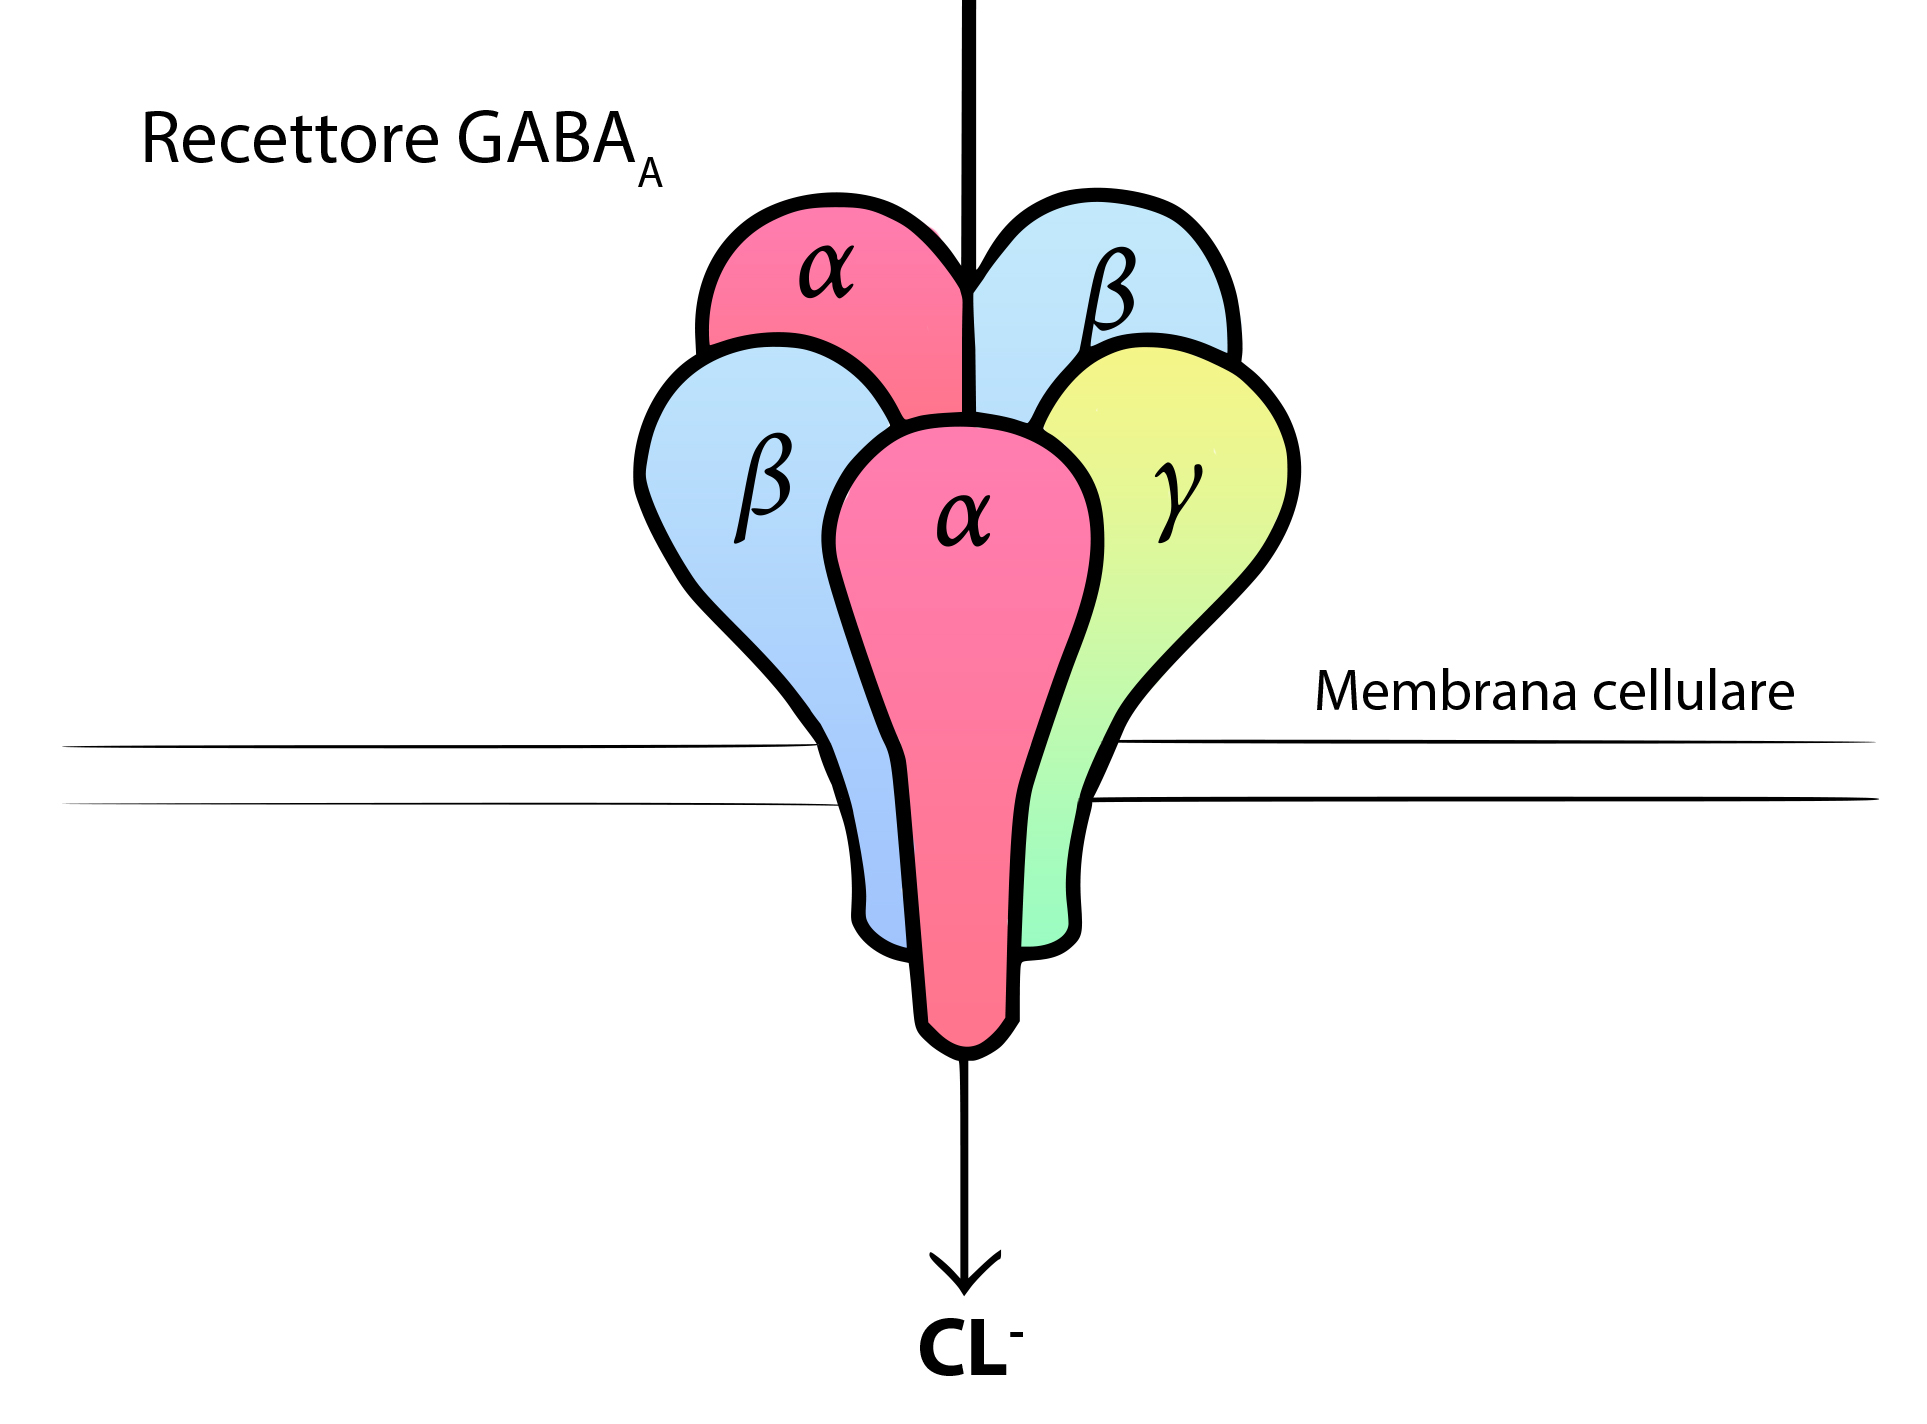
\includegraphics[width=0.6\textwidth]{Figure/GABAps.jpg}
    \caption{Recettore ionotropico GABA\ped{A}, adattata da \cite{vinkers2012}.}
    \label{fig:GABAps}
\end{figure}

\subsection*{Farmacocinetica}

Uno dei motivi per cui il propofol è ampiamente utilizzato riguarda proprio le sue favorevoli caratteristiche farmacocinetiche: ha infatti un esordio d'azione estremamente rapido (30-45 secondi) ed un altrettanto rapido risveglio (5-15 minuti dopo singolo bolo, più lento in caso di infusione continua o boli multipli) \cite{Simeupsedazione, Uptodatepharmacology}. Si tratta di una molecola liposolubile, che supera la barriera ematoencefalica; in soluzione assume un aspetto lattescente e può essere somministrata solo per via endovenosa. Nel momento dell'iniezione può causare bruciore locale, che può essere prevenuto utilizzando una vena di calibro maggiore o diluendo a metà il propofol con soluzione fisiologica (per una concentrazione di 5 mg/mL) \cite{Simeupsedazione}. 

\subsection*{Posologia}

Viene somministrato con un dosaggio di 1-2 mg/kg come bolo iniziale d'induzione, seguito da successivi boli multipli da 0.5 a 1 mg/kg ogni 2-3 minuti. Per le procedure più lunghe può anche essere utilizzato in infusione continua.
La dose massima è di 10 mg/kg totali per procedura \cite{Simeupsedazione}.

\subsection*{L'associazione con la ketamina}

Se la procedura è dolorosa il propofol può essere dato in combinazione con la ketamina, che oltre ad avere un'importante azione analgesica controbilancia gli effetti ipotensivo e bradicardizzante del propofol. Esistono in commercio delle formulazioni chiamate \emph{ketofol} con diversi rapporti di ketamina e propofol; tra i vantaggi risalta anche una minor incidenza di vomito e agitazione al risveglio, rispetto alla somministrazione della sola ketamina \cite{Simeupsedazione}. %poiché l'effetto combinato permette di risparmiare ketamina .

\subsection*{Effetti collaterali}

I principali effetti collaterali del propofol sono rappresentati dalla depressione respiratoria e dalla conseguente apnea, che dipendono dal dosaggio, dalla velocità di somministrazione e dalla risposta soggettiva del paziente. Inoltre, il propofol può determinare ipotensione e più raramente bradicardia \cite{propofolsafety2010}.
Un altro temibile quanto raro effetto avverso è costituito dalla \emph{propofol infusion syndrome}, potenzialmente fatale e documentata sia negli adulti che nei bambini \cite{Propofolinfusionsyndrome2019}. Si tratta di un insieme di segni e sintomi che si verifica in pazienti critici, che ricevono propofol in infusione a dosaggi elevati (> 5 mg/kg/h) o per un periodo prolungato (> 48h) ed è caratterizzata dalla presenza di una o più delle seguenti alterazioni, non spiegabili altrimenti: acidosi metabolica, rabdomiolisi, variazioni elettrocardiografiche associate o meno ad AKI, iperkaliemia, dislipidemia, scompenso cardiaco, febbre, elevazione degli enzimi epatici o del lattato. 

\section{Ketamina}

La ketamina è un farmaco anestetico dissociativo derivato dalla fenilciclidina con potenti proprietà sedative, analgesiche ed amnesiche. \`E stato introdotto in commercio per la prima volta nel 1970 e da allora viene largamente utilizzato per lo più in ambito anestesiologico, pur possedendo un'ampia gamma di possibili applicazioni cliniche \cite{Ketamineapplication2019}: dal trattamento del dolore cronico, anche in pazienti oncologici, al trattamento del disturbo depressivo maggiore, grazie ai suoi effetti antidepressivo ed antisuicidario. Inoltre, mentre rimane controverso il suo ruolo nel trattamento dell'asma, sono riconosciute le sue azioni antinfiammatoria ed immunomodulatrice, a cui si aggiungono quella antiproliferativa ed apoptotica, che vengono studiate con interesse per la ricerca sulla soppressione tumorale.

\subsection*{Farmacodinamica}

La ketamina è un farmaco che porta il paziente in uno stato dissociativo, simile alla trance, in cui l'individuo rimane parzialmente vigile ma con una depressione della consapevolezza: mantiene infatti gli occhi aperti ma non interagisce con l'ambiente circostante e non percepisce dolore. A differenza di altri farmaci non presenta un \emph{continuum della sedazione}, piuttosto l'effetto è presente o assente a seconda del dosaggio. Viene scelta per la sua ottima capacità analgesica e l'alto profilo di sicurezza, in quanto permette il mantenimento dei riflessi protettivi delle vie aeree e non deprime il centro del respiro; inoltre dal punto di vista cardiovascolare aumenta la frequenza cardiaca e la pressione arteriosa \cite{Krauss2006}. 
\\La ketamina esercita le sue proprietà attraverso l'interazione con diversi recettori. Tuttavia, la maggior parte degli effetti sono dovuti al blocco dei recettori NMDA (\emph{N-Metil-D-Aspartato}), ai quali il farmaco si lega come antagonista non competitivo. Si tratta di canali ionici glutammatergici permeabili agli ioni calcio, i quali normalmente sono implicati nell'attivazione di diversi pathway intracellulari \cite{Zanos2018}.
\\La ketamina esiste sotto forma di due enantiomeri\footnote{Sono isomeri ottici, ovvero entità molecolari speculari e non sovrapponibili.}: levogiro (S) e destrogiro (R). La forma levogira ha un maggior attività anestetica ed analgesica, favorisce una miglior immobilità del paziente e un recupero più rapido, mentre la forma destrogira è più efficace per l'uso antidepressivo \cite{Simeupsedazione}.

\subsection*{Farmacocinetica}

La ketamina è altamente liposolubile, si distribuisce ai tessuti periferici e supera rapidamente la barriera ematoencefalica. Viene preferenzialmente somministrata per via endovenosa o intramuscolare ma, seppur con una biodisponibilità inferiore, può essere utilizzata anche attraverso altre vie: intranasale, rettale ed orale \cite{Simeupsedazione, Ketamineapplication2019}. 
\\La ketamina viene metabolizzata per l'80\% dal fegato in norketamina, che mantiene un terzo delle proprietà della molecola originale, per poi venir eliminata per via urinaria. 
\\Per via endovenosa ha un inizio d'azione molto rapido, che avviene entro 1-2 minuti dalla somministrazione, anche la durata è breve (10-15 minuti) con un tempo di risveglio di circa 30-60 minuti \cite{Uptodatepharmacology}. Mentre la somministrazione per via intramuscolare ha un inizio d'azione di 10-15 minuti e una durata della sedazione di 30-40 minuti \cite{Berkenbosch2015}.

\subsection*{Indicazioni}

Questo farmaco viene comunemente utilizzato sia in urgenza che in elezione. Viene scelto principalmente per procedure dolorose e di breve durata, quali la riduzione di una frattura o la sutura di una ferita. Può essere usato anche in combinazione con il propofol, al fine di aumentare il grado di sedazione e migliorare il profilo emodinamico, durante procedure d'elezione, quali colonscopie o aspirati midollari. Inoltre, per le sue caratteristiche neuroprotettive, viene spesso scelta in caso di intubazione d'urgenza di pazienti con traumi cranici severi \cite{Simeupsedazione}.

\subsection*{Posologia}

Una caratteristica distintiva della ketamina consiste nell'avere una relazione diretta tra la dose e l'effetto che si vuole ottenere, non esiste infatti per questo farmaco un \emph{continuum} tra i diversi livelli di sedazione. Vengono riportati nella seguente tabella \ref{tab:1} i dosaggi per via endovenosa associati all'intento terapeutico che si vuole raggiungere.

\bgroup
\def\arraystretch{1.5}
\begin{table}[!h]
    \centering
    \begin{tabular}{|l|l|}
       Scopo terapeutico     & Dosaggio \\ \hline
       Analgesia & 0.1-0.3 mg/kg  \\
       Aspetto ricreazionale & 0.3-0.6 mg/kg \\
       Sub-dissociativa & 0.4-0.8 mg/kg \\
       Analgosedazione & 0.8-1 mg/kg 
    \end{tabular}
    \caption{Adattata da \cite{Simeupsedazione}.}
    \label{tab:1}
\end{table}
\egroup

%\bigskip

La posologia relativa alle altre vie di somministrazione è, invece la seguente: 
\begin{itemize}
    \item via intramuscolo: 4-5 mg/kg
    \item via intranasale: 1-3 mg/kg (massimo 1 mL per narice)
    \item via orale: 5-10 mg/kg
\end{itemize}

\subsection*{Effetti collaterali}

Il principale svantaggio di questo agente farmacologico è rappresentato dalla lunga lista di effetti avversi che possiede. Il più temibile è rappresentato dal laringospasmo, che si può verificare soprattutto in seguito a stimolazione delle prime vie aeree, conseguente ad esempio a scialorrea, altro effetto collaterale della ketamina, oppure a gastroscopia. Inoltre, l'utilizzo di alte dosi di ketamina può causare allucinazioni e deliri al risveglio, il cosiddetto \emph{bad trip}. Si tratta di episodi solitamente autorisolventi in poche ore ma spiacevoli per il paziente e i genitori; i casi più intensi possono beneficiare della somministrazione di benzodiazepine \cite{Simeupsedazione}. Altri effetti collaterali minori ma frequenti (8\%) sono rappresentati dalla nausea e dal vomito, che possono essere prevenuti tramite la somministrazione di ondansetron (0.15 mg/kg), un antiemetico \cite{Uptodatepharmacology}. Inoltre, la ketamina può determinare la comparsa di nistagmo orizzontale, un effetto privo di significato clinico \cite{Simeupsedazione}. 
\\L'insorgenza di reazioni avverse è più frequente se il farmaco è stato somministrato a dosaggi superiori o inferiori a quelli terapeutici, mentre la combinazione con il propofol porta ad una minor incidenza di agitazione al risveglio e vomito, poiché permette di ridurre le dosi di ketamina utilizzata durante la procedura \cite{Simeupsedazione, Shah2011}. 

\subsection*{Controindicazioni}

L'uso della ketamina è controindicato in termini assoluti nei lattanti con meno di tre mesi di vita, che risultano, anche per motivi anatomici, più soggetti a reazioni respiratorie gravi \cite{Zanos2018}; negli affetti da schizofrenia, in quanto gli effetti psicoattivi della ketamina possono esacerbarne i sintomi; infine nei pazienti che hanno avuto precedentemente gravi reazioni collaterali \cite{Uptodatepharmacology}.
\\Altre controindicazioni relative, invece, riguardano soggetti con: instabilità delle vie aeree, infezioni o patologie polmonari attive, patologie cardiovascolari tra cui ipertensione, angina o scompenso cardiaco, porfiria, tireopatie e assunzione di farmaci per la tiroide, che possono aumentare l'effetto simpaticomimetico. Infine l'età compresa tra 3 e 12 mesi, l'aumentata pressione intracranica dovuta a lesioni occupanti spazio e l'aumentata pressione intraoculare, conseguente a glaucoma od altre lesioni oculari, sono controindicazioni attualmente messe in dubbio e non più suffragate \cite{Green2011, Simeupsedazione}.   

\section{Midazolam}

Il midazolam è una benzodiazepina a breve durata d'azione, che possiede proprietà ansiolitiche, sedative, amnesiche\footnote{Con interessamento solo della memoria anterograda, non viene invece influenzata quella retrograda.}, anticonvulsivanti, ipnoinducenti e miorilassanti; non possiede tuttavia azione analgesica \cite{Krauss2006}. 
\\ \`E il farmaco più comunemente usato per la sedazione minima (o ansiolisi) in ambito pediatrico, inoltre può essere utilizzato con un adeguato profilo di sicurezza fino a un livello di sedazione moderato \cite{Manso2019}. Per una maggior profondità, invece, è preferibile l'associazione con altri agenti farmacologici, al fine di prevenirne gli effetti avversi dose-correlati.

\subsection*{Farmacodinamica}

Il meccanismo d'azione delle benzodiazepine è dovuto al potenziamento dell'attività inibitoria neuronale, fisiologicamente esercitata dal legame tra il neurotrasmettitore GABA e i suoi recettori. Esistono due tipi di recettori per l'acido $\gamma$-amminobutirrico: i recettori ionotropici GABA\ped{A} e i recettori metabotropici GABA\ped{B}. Le benzodiazepine si legano alla subunità $\gamma$ dei recettori GABA\ped{A} in modo esclusivo e con una maggior affinità rispetto al neurotrasmettitore endogeno, che invece si lega alla subunità $\beta$ degli stessi\footnote{Le subunità del recettore GABA\ped{A} sono mostrate in figura \ref{fig:GABAps}.}. Ne consegue un maggior effetto di depressione neuronale, grazie allo stesso meccanismo descritto poco sopra nella sezione di farmacodinamica del propofol \cite{Olkkola2008}. 
\\Come schematicamente rappresentato nella figura \ref{fig:benzo}, gli effetti clinici si susseguono dall'ansiolisi alla sedazione fino all'ipnosi in relazione al grado di saturazione dei recettori GABA\ped{A}, che dipende a sua volta dalla concentrazione ematica del farmaco. 

\begin{figure}[t]
    \centering
    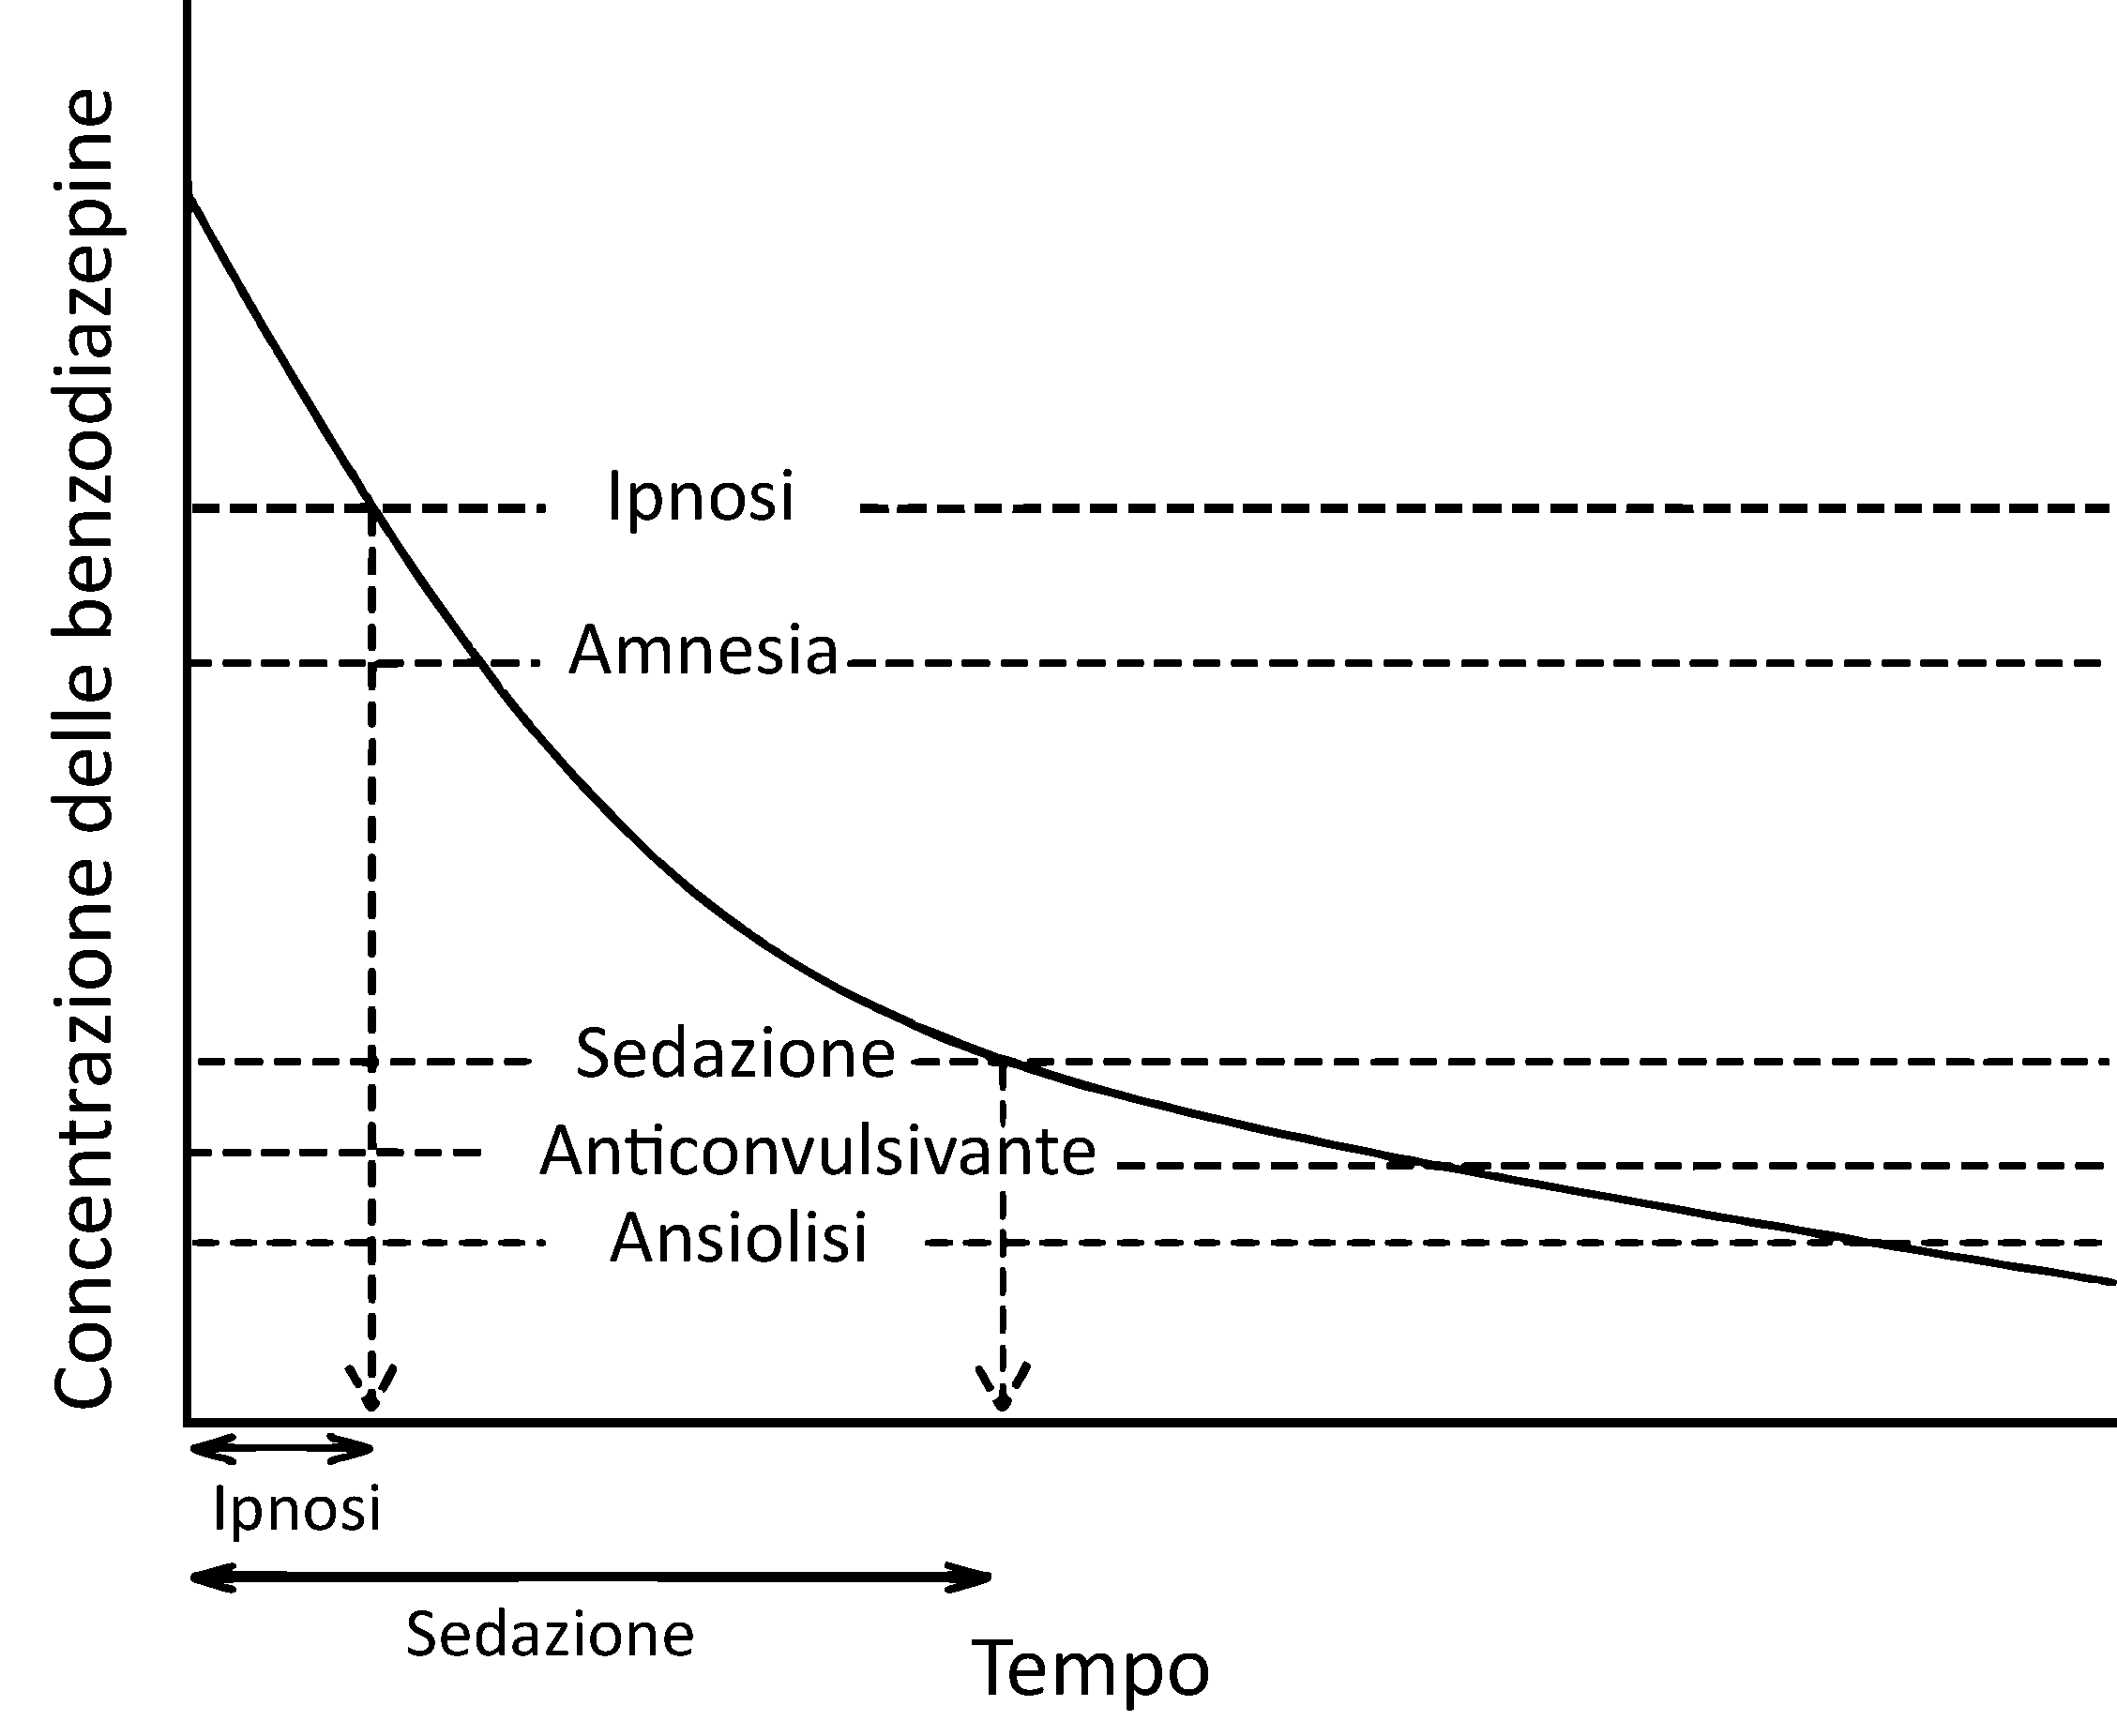
\includegraphics[width=0.7\textwidth]{Figure/BENZOpdf.pdf}
    \caption{Relazione tra la concentrazione ematica delle benzodiazepine e i diversi effetti clinici ottenibili, immagine adattata da \cite{Olkkola2008}.}
    \label{fig:benzo}
\end{figure}

\subsection*{Farmacocinetica}

Uno dei principali punti di forza del midazolam è rappresentato dalla sua struttura molecolare altamente lipofilica. Per tale ragione, da una parte supera con facilità la barriera ematoencefalica, dall'altra raggiunge un'elevata biodisponibilità anche tramite vie di somministrazione alternative a quella endovenosa ---intranasale, orale, rettale ed intramuscolare---, permettendone l'utilizzo in assenza di un accesso venoso \cite{Krauss2006}. Ha inoltre anche altri vantaggi: raggiunge rapidamente il picco plasmatico, da 1-3 minuti per via endovenosa a 20-50 minuti dopo assunzione orale, ed ha una breve durata d'azione, di circa 30-60 minuti \cite{Simeupsedazione, Uptodatepharmacology}. 
Quest'ultima è dovuta alla veloce metabolizzazione del farmaco, ancor più accentuata nei bambini \cite{Payne1989}: il midazolam viene idrossilato a livello epatico dal citocromo P450 in due metaboliti, ancora farmacologicamente attivi, che vengono a loro volta glucuroconiugati per formare prodotti inattivi, escreti poi nelle urine \cite{Olkkola2008}. 

\subsection*{Indicazioni}

Questo agente farmacologico si rivela molto utile in tutte le procedure che richiedono l'ansiolisi del bambino, ad esempio per il posizionamento di un accesso venoso o per la sutura delle ferite. Inoltre, può essere utilizzato in associazione ad altri farmaci per la sedazione prima di manipolazioni ortopediche, studi radiologici o procedure diagnostiche e/o terapeutiche più impegnative \cite{Simeupsedazione, Olkkola2008}. 

\subsection*{Posologia}

I dosaggi del midazolam per le vie di somministrazione più comunemente adottate sono i seguenti \cite{Simeupsedazione}: 
\begin{itemize}
    \item via orale: 0.5 mg/kg (dose massima 20 mg)
    \item via intranasale: 0.2-0.8 mg/kg (dose massima 15 mg)\footnote{Il volume massimo utilizzabile per narice è di 1 mL, perciò nei bambini più grandi risulta utile l'impiego di formule concentrate associate a premedicazione con lidocaina spray per ridurre il bruciore locale causato dall'applicazione.}
    \item via endovenosa: 0.1 mg/kg (dose massima 5 mg)
\end{itemize}

\subsection*{Effetti collaterali}

Dal punto di vista respiratorio il midazolam può causare due complicazioni: da una parte può ridurre il tono muscolare aumentando il rischio di ostruzione delle vie aeree superiori, dall'altra può inibire il fisiologico stimolo respiratorio all'ipossia, determinando una possibile depressione ventilatoria dose-correlata fino all'apnea. Per tali ragioni è sconsigliabile l'utilizzo in combinazione con altri agenti che deprimono il centro del respiro. 
Inoltre, esercita un'azione sull'apparato cardiovascolare, riducendo in maniera modesta la pressione arteriosa e aumentando la frequenza cardiaca \cite{Olkkola2008}. 
\\Un altro evento comunemente descritto in letteratura, con un'incidenza tra l'1$\%$ e il 10$\%$, riguarda il \emph{midazolam-induced paradox phenomenon} \cite{Weinbroum2001}: occasionalmente il midazolam, anziché esercitare un'azione calmante e sedativa, determina crisi di agitazione, pianto inconsolabile, iperattività, ostilità ed aggressività fino ad arrivare a comportamenti violenti. Sia le reazioni paradosse che la depressione respiratoria possono essere revertite in pochi minuti tramite la somministrazione del flumazenil, ovvero un antagonista competitivo delle benzodiazepine con alta affinità per il recettore GABA\ped{A}, che può essere somministrato efficacemente sia per via endovenosa che per via intranasale. \`E importante monitorare strettamente il bambino nelle ore successive la somministrazione, poiché, oltre ad avere un inizio d'azione molto rapido (1-2 minuti), presenta anche un'emivita breve, inferiore a quella del midazolam, con possibile ricomparsa dei sintomi \cite{Simeupsedazione, Uptodatepharmacology}.


\section{Dexmedetomidina}

La dexmedetomidina è un farmaco relativamente recente\footnote{\`E stata approvata nel 2008 dalla \emph{Food and Drug Administration} per l'utilizzo al di fuori della terapia intensiva \cite{Simeupsedazione, Uptodatepharmacology}.}, che esercita un'attività sedativa molto simile al sonno fisiologico; inoltre ha proprietà ansiolitica, moderatamente analgesica, simpaticolitica ed incide con effetti minimi sul centro del respiro \cite{Mahmoud2015}.

\begin{figure} [t]
    \centering
    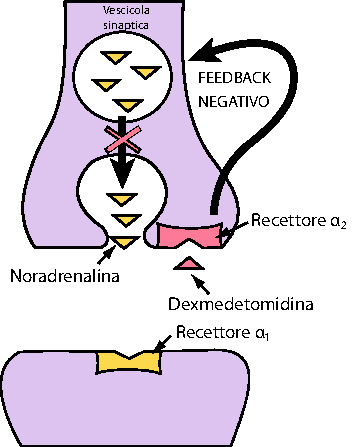
\includegraphics[width=0.4\textwidth]{Figure/dexfigpdf.pdf}
    \caption{Meccanismo d'azione della dexmedetomidina, adattata da \cite{Gertler2001}.}
    \label{fig:DEX}
\end{figure}

\subsection*{Farmacodinamica}

La dexmedetomidina è un agonista altamente selettivo per i recettori $\alpha$\ped{2} e possiede un'ampia gamma di proprietà farmacologiche, riflettenti la distribuzione ubiquitaria di tali recettori nel nostro organismo \cite{Keating2015}. Come rappresentato nella figura \ref{fig:DEX}, i recettori $\alpha$\ped{2}, una volta stimolati, inibiscono il rilascio dei neurotrasmettitori endogeni ---adrenalina e noradrenalina---, realizzando un blocco dell'attività simpatica. Gli effetti sedativo ed ipnotico della dexmedetomidina sono dovuti all'attivazione di questi recettori a livello del locus ceruleo nel tronco cerebrale, con conseguente soppressione della trasmissione dello stimolo neuronale e promozione delle vie endogene del sonno. Il paziente sviluppa, quindi, uno stato molto simile alla seconda fase del sonno non-REM fisiologico, da cui risulta facilmente risvegliabile, caratteristica unica tra i sedativi attualmente disponibili \cite{Weerink2017, Gertler2001}.
La lieve azione analgesica, invece, è dovuta alla stimolazione dei recettori $\alpha$\ped{2} a livello delle corna dorsali del midollo spinale, con inibizione della via nocicettiva e riduzione del rilascio di sostanza P e glutammato, implicati nella percezione del dolore \cite{Weerink2017}. Inoltre, mentre dal punto di vista respiratorio la dexmedetomidina non determina effetti clinicamente significativi e consente di mantenere il normale stimolo ventilatorio, dal punto di vista cardiovascolare produce una risposta emodinamica bifasica, dipendente dalla concentrazione ematica del farmaco. Infatti, ad alte dosi si verifica ipertensione accompagnata ad una riduzione della frequenza cardiaca: l'azione agonista sui recettori $\alpha$\ped{2} presenti a livello della muscolatura liscia vascolare provoca vasocostrizione, con conseguente aumento pressorio ed attivazione del riflesso barocettivo\footnote{Consiste nella stimolazione, in seguito ad un repentino incremento della pressione arteriosa, di neuroni specializzati localizzati principalmente a livello dell'arco aortico e dei seni carotidei, che forniscono un feedback negativo, causando una diminuzione della frequenza cardiaca e favorendo l'omeostasi pressoria.}. Quando invece la concentrazione ematica del farmaco scende, ad esempio qualche minuto dopo la somministrazione di un bolo per via endovenosa, inizia una fase ipotensiva, in quanto prevale l'attività simpaticolitica associata alla vasodilatazione indotta dal legame con i recettori presenti a livello endoteliale \cite{Weerink2017}. 

\subsection*{Farmacocinetica}

La dexmedetomidina è un farmaco ad elevata liposolubilità, che può essere somministrato, con garanzia di un'adeguata biodisponibilità, tramite diverse vie: endovenosa, intramuscolare, intranasale e sottolinguale. Inoltre, ha un inizio d'azione piuttosto rapido, seppur più lento rispetto ad altri agenti sedativi, con un'emivita di distribuzione di circa 6 minuti. A livello plasmatico si trova per il 96$\%$ legata alle proteine, soprattutto all'albumina, e viene metabolizzata quasi interamente a livello epatico grazie al citocromo P450\footnote{Per tale ragione andrebbe utilizzata con cautela nei soggetti con insufficienza epatica, prendendo in considerazione un dosaggio di mantenimento ridotto \cite{Keating2015}.}; i prodotti derivanti dall'attività epatica vengono poi escreti con le urine con un'emivita di eliminazione di circa 2 ore \cite{Gertler2001, Keating2015, Weerink2017}. 

\subsection*{Indicazioni}

Questo agente farmacologico può essere utilizzato sia in terapia intensiva che al di fuori della sala operatoria con un ampio numero di possibili applicazioni perioperatorie e periprocedurali \cite{Mahmoud2015}. Considerate le sue caratteristiche e il suo elevato profilo di sicurezza risulta particolarmente utile per le procedure non dolorose, quali l'ecocardiografia e l'elettroencefalogramma\footnote{La dexmedetomidina, a differenza di altri agenti sedativi, non determina artefatti elettrici.}, soprattutto nei bambini piccoli o non collaboranti. Inoltre, può essere usato in associazione al midazolam per l'esecuzione di esami radiologici, come la RM, oppure in combinazione con altri farmaci per lo svolgimento di procedure diagnostiche o terapeutiche maggiori \cite{Simeupsedazione}. Alcuni studi lo valutano superiore al midazolam in affidabilità, analgesia e soddisfazione sia del medico che del paziente per le sedazioni procedurali \cite{Barends2017, Lin}.

\subsection*{Posologia}

I dosaggi relativi alle diverse vie di somministrazione sono i seguenti \cite{Simeupsedazione, Uptodatepharmacology}: 

\begin{itemize}
    \item via endovenosa: bolo di 1-2 \unit{\ug/kg} in 10 minuti + infusione continua a 0.1 \unit{\ug/kg/h}
    \item via intranasale\footnote{Ha un inizio d'azione di circa 30-50 minuti dopo la somministrazione ed una durata di 1-2 ore \cite{Simeupsedazione}.}: 3-4 \unit{\ug/kg} (dose massima 100 \unit{\ug}) + possibilità di dose \emph{rescue} dopo 30 minuti di 1 \unit{\ug/kg}
    \item via intramuscolare: 4 \unit{\ug/kg} (dose massima 200 \unit{\ug})
    \item via sottolinguale\footnote{Solo se il bambino è collaborante e non deglutisce il farmaco perché la biodisponibilità in tal caso si ridurrebbe al 16$\%$ \cite{Weerink2017}.}: 3-4 \unit{\ug/kg}
\end{itemize}

\subsection*{Effetti collaterali}

La dexmedetomidina è un farmaco molto sicuro: presenta complessivamente\footnote{Sulla base di un ampio studio osservazionale prospettico su oltre 13.000 bambini \cite{Sulton2016}.} meno del 4$\%$ di effetti avversi, di cui gravi solo meno del 0.3$\%$. Infatti, questo farmaco non altera il fisiologico stimolo respiratorio e i più frequenti effetti descritti, che interessano principalmente l'apparato cardiovascolare, nella maggior parte dei casi non necessitano di intervento farmacologico. Si può verificare una transitoria ipertensione nel momento del picco plasmatico, seguita talvolta da ipotensione, correggibile con boli di soluzione fisiologica; più raramente può invece manifestarsi bradicardia, che si può eventualmente trattare con atropina \cite{Sulton2016}. Per tali motivi è controindicata nei bambini che assumono farmaci $\beta$-bloccanti o digitalici, nei soggetti con patologie della conduzione cardiaca o in cui una ridotta gittata o un'aumentata pressione polmonare risulterebbero mal tollerate (ad esempio nello scompenso cardiaco o nello shock settico) \cite{Uptodatepharmacology, Simeupsedazione}. 